\documentclass[a4paper, 14pt]{article}
\usepackage{graphicx}
\usepackage{amsfonts}
\usepackage{fancyhdr}
\usepackage{cite}
\usepackage{color}
\definecolor{light-gray}{gray}{0.3}
\newcommand{\HRule}{\rule{\linewidth}{0.5mm}}
\title{\bf Assignment 04}
\author{Xugang Zhou \\ Fangzhou Yang \\ Yuwen Chen}
\pagestyle{fancy}
\lhead{{\bf Distributed Algorithm}\\WS 2013/14, Prof. Dr.-Ing. Jan Richling}
\rhead{Assignmen 02}
\renewcommand{\headrulewidth}{0.4pt}
\begin{document}
\begin{titlepage}
\begin{center}
\vfill
\textsc{\LARGE Distributed Algorithm}\\[1.5cm]
\textsc{\Large }\\[0.5cm]

\HRule \\[0.4cm]
{\huge \bfseries Assignment 04}\\[0.4cm]
\HRule \\[1.5cm]
\begin{minipage}{0.4\textwidth}
\begin{flushleft} \large
\large{\textbf{Group 11}}
\end{flushleft}
\end{minipage}
\begin{minipage}{0.4\textwidth}
\begin{flushright} \large
\begin{tabular}{ll}
Xugang \textsc{Zhou} & 352032\\
Fangzhou \textsc{Yang} & 352040\\
Yuwen \textsc{Chen} & 352038
\end{tabular}
\end{flushright}
\end{minipage}
\vfill
{\large \today}\\
\end{center}
\end{titlepage}
\thispagestyle{fancy}

\section{Lamport}

Given the original FIFO case below (from the lecture's slide):\\
\centerline{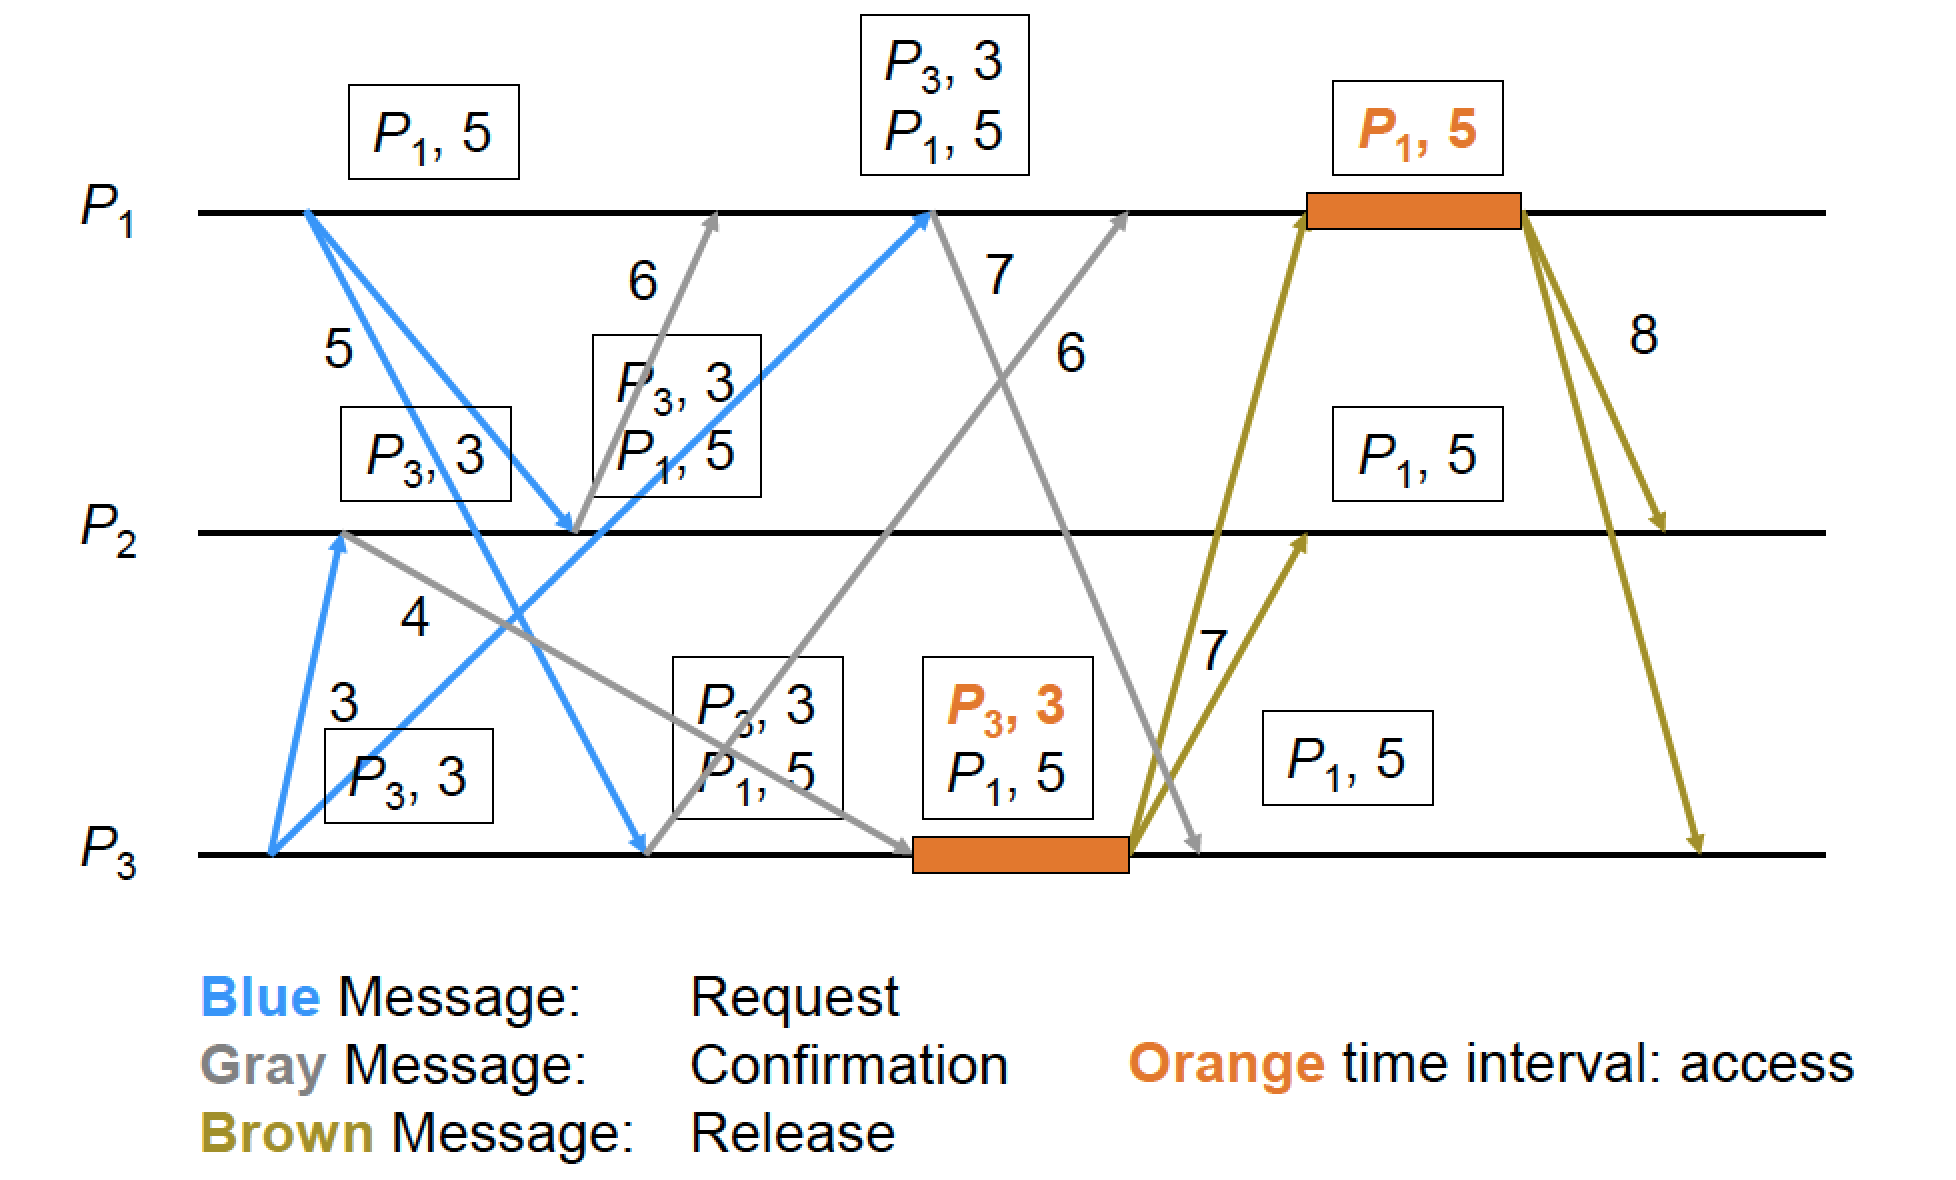
\includegraphics[width=10cm]{LamportExample.png}}
If this algorithm runs in a non-FIFO channel environment, {\color{light-gray}Confirmation}
message of $P_3$ to $P_1$ could arrive ealier than $P_3$'s
{\color{blue}Request} message. Then for $P_1$, it would be confused
and access the resource which is currently been using by $P_3$. \cite{Lamport1978}

\section{Ricart and Agrawala}

\begin{itemize}
\item[a)] Ricart and Agrawala have been shown that the deadlock is impossible. \cite{Ricart1981} \\
  If deadlock is possible, then all nodes should be waiting for one or more
  confirmations. Since the only possibility that a confirmation is
  being waited by one node is that this node's request is deferred by
  some other node. \\
  So, there should be a circle of nodes, each one sent its request to
  its next but waits for another reply. In this situation, the
  sequence number / node number pair of the request recieved by each
  node should be greater than its own, which, in a circle, is
  impossible.\\ 
\item[b)] In the original algorithm, the node should wait for $n-1$
  confirmations before it can access the resource. In order to allow
  (maximum) $k \in \mathbb{N}$ nodes at once, we can change the rule:
  {\bf A node could access the resource after it receives $n-k$
  confirmations.} 
\end{itemize}

\section{Maekawa}
\begin{itemize}
\item[a)] Yes, the algorithm is still feasible. As shown in
  \cite{Maekawa1985}, if $n$ is not a square of an integer, we can
  create a degenerate grid. Which means that we could find a $m > n$
  which $m$ is a square, and construct the set using $m$. Then we can
  replace numbers from $n$ to $m$ by numbers below $n$ respectively
  and remove the sets constructed for nodes greater than $n$.
\item[b)] In triangular case, there are even less messages needed to
  be sent because each sets contains less nodes than in quadratic
  case. But since every two sets intersect with only one nodes, so
  triangular arrangement is less robust than the quadratic's.\\
\cite{Maekawa1985} also shows that $N = K(K - 1) + 1$, for ($N$ is the
number of nodes, $K$ is the number of nodes in one set). \\
When $K - 1$ is a power of some prime, finding $S_i$ is equivalent to
find the finite projective plane of $N$ points. For other $K$, we can
create a degenerated set just like the previous sub-problem. Even if
$N$ can not be represented by $N = K(K - 1) + 1$ for any $K$, similar
method to create a degenerated set could be applied.
\end{itemize}
\newpage
\bibliographystyle{plain}
\bibliography{DAAssignment04}{}
\end{document}


